% Created 2016-12-16 Fr 23:12
% Intended LaTeX compiler: pdflatex
\documentclass[11pt]{llncs}

\tolerance=1000

\usepackage[T1]{fontenc}
%% % \usepackage[longnamesfirst,sort,nonamebreak]{natbib}
%% \usepackage[normalem]{ulem}
%% \usepackage[table]{xcolor}
\usepackage[utf8]{inputenc}
%% \usepackage{amsmath}
%% \usepackage{amssymb}
%% \usepackage{amstext}
%% \usepackage{array}
%% \usepackage{authblk}
%% \usepackage{caption}
%% \usepackage{color}
%% \usepackage{epsfig} % for postscript graphics files
%% \usepackage{fixltx2e}
%% \usepackage{float}
%% % \usepackage{fullpage}
%% \usepackage{graphics} % for pdf, bitmapped graphics files
\usepackage{hyperref}
%% \usepackage{latexsym}
%% \usepackage{lmodern}
%% \usepackage{longtable}
%% \usepackage{makeidx}  % allows for indexgeneration
%% \usepackage{marvosym}
%% \usepackage{multirow}
%% \usepackage{subcaption}
%% % \usepackage{subfigure}
%% \usepackage{textcomp}
%% \usepackage{titling}
%% \usepackage{wasysym}
%% \usepackage{wrapfig}

% \renewcommand{\familydefault}{\sfdefault}
% \parindent10pt

\usepackage[style=authoryear,backend=biber,bibencoding=utf8,natbib]{biblatex}
\bibliography{actinf}
\addbibresource{actinf.bib}

\usepackage{tikz}
\usetikzlibrary{arrows,positioning}

\graphicspath{{./img/}{img/}}
\DeclareGraphicsRule{.ps.gz}{eps}{.ps.bb}{`zcat #1}



\newcommand{\blg}[1]{
(\textcolor{red}{blg. #1})
}

%------------------------------------------------------------------------- 
% args: <label> <fileName> <caption> <scale>
\newcommand{\figone}[4]{
  \begin{figure}[ht]
  \begin{center}
  \includegraphics[scale=#4]{#2}
  \begin{sl}
  \caption{\label{#1}#3}
  \end{sl}
  \end{center}
  \end{figure}
}
%\figone{fig1}{figura.pdf}{caption de la figura}{5}



%------------------------------------------------------------------------- 
% args: <label> <fileName> <caption> <scale>
\newcommand{\figoneforced}[4]{
  \begin{figure}[h!t]
  \begin{center}
  \includegraphics[scale=#4]{#2}
  \begin{sl}
  \caption{\label{#1}#3}
  \end{sl}
  \end{center}
  \end{figure}
}
%\figone{fig1}{figura.pdf}{caption de la figura}{5}




%to insert a tikz fig in the local directory plus /figs
% args: <label> <fileName> <caption> 
\newcommand{\figtikz}[4]{
\begin{figure}[ht]
\begin{center}
\scalebox{#4}{\input{figs/#2}}
\begin{sl}
\caption{\label{#1}#3}
\end{sl}
\end{center}
\end{figure}
}
%------------------------------------------------------------------------- 

%to insert a tikz fig in the local directory plus /figs
% args: <label> <fileName> <caption> acuerdate esta instruccion esta mal
\newcommand{\figtikzF}[4]{
\begin{figure}[h!t]
\begin{center}
\scalebox{#4}{\input{figs/#2}}
\begin{sl}
\caption{\label{#1}#3}
\end{sl}
\end{center}
\end{figure}
}
%------------------------------------------------------------------------- 



% \title{Predictive Processing Model for an Autonomous Agent}
\title{Predictive Processing Model for an Autonomous Agent}
\titlerunning{Predictive Processing Model}  % abbreviated title (for running head)


\author{Bruno Lara\thanks{bruno.lara@uaem.mx}\inst{1} \and Alejandra
  Ciria \inst{2}
  \and Guido Schilacci \inst{3} \and Oswald Berthold \inst{3}}

%% \renewcommand\Authands{ and }

\institute{Cognitive Robotics Group, Center for Science Research,
  Universidad Aut\'onoma del Estado de Morelos, Cuernavaca, M\'exico
  \and Psychology Faculty, Universidad Nacional Aut\'onoma de
  M\'exico, M\'exico
  \and Adaptive Systems Group, Department of Computer Science,
  Humboldt-Universitaet zu Berlin, Berlin, Germany
}

% \author{Guido, Bruno, Alejandra, Esau, Oswald}
% \date{\today}
%% \hypersetup{
%%  pdfauthor={Guido, Bruno, Alejandra, Esau, Oswald},
%%  pdftitle={Predictive Processing Model for an Autonomous Agent},
%%  pdfkeywords={},
%%  pdfsubject={},
%%  pdfcreator={Emacs 24.3.1 (Org mode 9.0.1)}, 
%%  pdflang={English}}

\begin{document}

\maketitle

\begin{abstract}
We examine an approach to autonomous acquisition of motor skills and
behaviour using computational models. Our focus is on the role of
\emph{predictive coding} of sensorimotor data. Based on the apparent
prevalence of predictive coding in animal's brains, we follow the
hypothesis that predictive coding provides systematic and unique
characteristics facilitating learning and exploration.
% Short description of the project
\end{abstract}



\section{Introduction}
\label{intro}

Motor control for autonmous agents that need to learn some things
about the relations between observable quantities.


Our work is motivated by wanting to better understand how animals such as
ourselves are able to change, adjust and invent behaviour as
efficiently as they do. We assume such understanding to be relevant
for building a theory of robots, guidelines for the synthesis of
artificial systems interacting with the real world.

Existing research has shown the problem to be quite challenging and
varied and many such variations have been examined. The task is to try
and systematize the phenomena by identifying functional principles
that are at work over wide ranges of organisms and mechanisms
\citep{pfeifer07}.

We examine a small set of such principles in combination: Predictive
coding, internal modelling, and top-down information flow. We start
with the principle of Predicitive Coding (PC) which is a coding scheme
encountered in the analysis of nervous systems. The principle says
that of all input only that part of the input to a functional unit,
implemented by a layer or a module, which has not been predicted is
allowed to pass through for further processing. This quantity, usually
a vector, is the prediction error (PE).

The prediction error quantifies what the system doesn't know already
and is worthy of additional predictive modelling. PE combines external
(input complexity conditioned on output) and internal (model failures)
factors. Knowing the relation of model change to PE change allows to
infer particular sensorimotor contexts as driven by external
factors. Longterm PE behaviour can modulate adaptation, while
shortterm PE generally drives activity.

% ``inherent unpredictability''
% A possible hypothesis is .. damn it escaped me ..

Next is internal modelling (IM). IM is closely related to PE because
any prediction in fact requires a model. Such a model needs to map the
information from the past to the scope of prediction, usually one or a
few timesteps (1s).

Top-down information flow then says that experience, the apex of
decision making, is being driven or initiated by a prediction about
the next state. Only unpredicted (unmodelled) parts of the next
post-prediction measurements are being passed on.

%% Building on that and other existing concepts, the internal model
%% hypothesis (IMHT), and prediction / prediction error information flow
%% (PPEIF) we propose and analyze a simple model complying with the
%% principles.

We can take these three principles for the design of the proposed models:

\begin{itemize}

\item Discuss the change of terminology or dichotomies regarding:
  \begin{itemize}
  \item predictions/motor commands,
  \item forward models/inverse models/controllers/policies
  \item bottom level black box: different actual forward model (FM)
    representations via SOMs, kNN, RLS, GP, \ldots{}
  \item see discussion with antonio re: "it's just labels", underneath it is a raw
    network of signal flows putting observable quantities into
    relation to each other, from which apparent goal-driven behaviour
    (teleology) emerges
  \end{itemize}


\item Proprioceptive space: any embodied agent has to have a lowest
  level motor system. This is usually represented by a vector of motor
  angles, motor velocities, motor torques, etc but essentially it can be any
  given kind of controller. A controller in this sense implies a
  measurement and a prediction defined in the same space. This is the
  point at which we want to engange in interaction with the
  system.

\item The forward model is part of a larger building block, a
  generative model, mapping from control (goals) to to sensory
  consequences \citep{friston2011}.

\item The main flow of information is top-down, not bottom-up, and the
  forward flow of sensory information is replaced by the forward flow
  of prediction error \citep{clark2015}. FIXME: define top, botton,
  forward, etc?

\item Sensory prediction errors ($Err_{e(t)}$, $Err_{p(t)}$) are
  required for online state estimation (inference) and for optimizing
  (learning) the forward model \citep{friston2011}, or any kind of
  activity. 

\item Descending propioceptive predictions are equivalent to motor
  commands. Movement quash error at the level of spinal reflexes
  \citep{pickering2014}. Propioceptive predictions elicit motor
  actions, so motor commands are replaced by those
  propioceptive predictions \citep{clark2015}. $S^*_{p(t)}=M_{(t)}$.

\item Motor commands become descending predictions or propioceptive
  sensations, while their exteroceptive homologous become corollary
  discharges \citep{friston2011}.

\item Motor behaviours are predictions of propioceptive
  patterns. Motor control is just more top-down sensory prediction
  \citep{clark2015}. 

\item Action: results from our own predictions concerning the flow of
  sensations \citep{pickering2014}. 

\item High-level plans and intentions (prior beliefs) associate with
  sensory consequences and actions flow. This is, high level states
  into predicted sensory patterns \citep{pickering2014}.

\end{itemize}

%%%%%%%%%%%%%%%%%%%%%%%%%%%%%%%%%%%%%%%%%%%%%%%%%%%%%%%%%%%%%%%%%%%%%%%%%%%%%%%%
\section{Related}
\label{sec:orgf9aed21}

Long history, many models: control, development, RL, neuroscience, ...\ldots{}


%%%%%%%%%%%%%%%%%%%%%%%%%%%%%%%%%%%%%%%%%%%%%%%%%%%%%%%%%%%%%%%%%%%%%%%%%%%%%%%%
\section{Proposed Models}
\label{plan}

\subsection{General Models}

First two basic models and their difference in terms of learning
dynamics. Do any dynamic properties support or contradict biological
motor learning?

\subsection{M1}

The basic building block (BBB) contains an adaptive forward model
(predictor) whose output is the BBB's output. We assume direct
feedback from that module that the output is connected to. The BBB'
inputs are an explicit goal and the prediction error with respect to
the last prediction at ${t-1}$. These inputs taken together encode the
state. Thus the forward model should in principle be able to pick up
on different relations depending on the state. Graphical
representation is given in \autoref{fig:M1}.

\begin{figure}
  \centering
  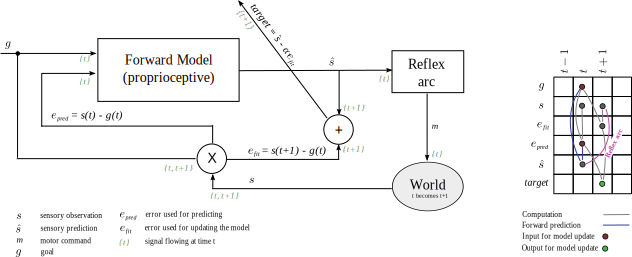
\includegraphics[width=0.9\textwidth]{img/mdl_prediction_error_and_goal.pdf}
  \caption{\label{fig:M1} Basic model M1.}
\end{figure}

\subsection{M2}

This modification of BBB M1 receives only the error as an input. The
model's graph is shown in \autoref{fig:M2}. This model will not be
able to distinguish between situations demanding different
predictions.

\begin{figure}
  \centering
  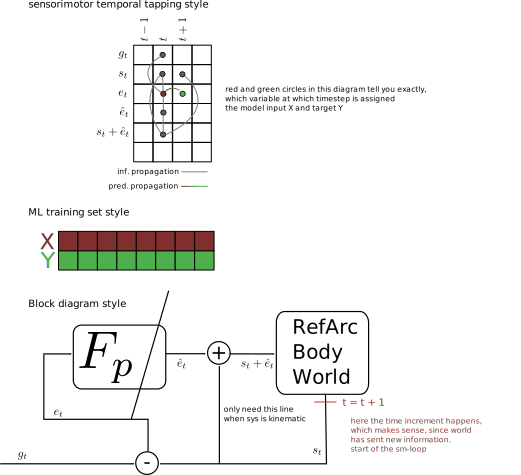
\includegraphics[width=0.9\textwidth]{img/mdl_prediction_error_only.pdf}
  \caption{\label{fig:M2} Basic model M2.}
\end{figure}

\subsection{Extended models connecting modalities}

Merge with alejandra's two versions (explicit update rule).

This model includes both propio and extero (Figs \ref{fig:basic1}
and \ref{fig:basic2}). The only difference is how the 
predictive error is calculated for the propioceptive information ($Err_{Pi(t)}$).

%\figtikz{fig:ltp}{fig_im_ltp}{Long term prediction}{0.9}


\figone{fig:basic1}{Integral_v3}{Model A}{0.8}
\figone{fig:basic2}{Integral_v4}{Model B}{0.8}

\subsection{Case Study Models}

In the example to simulate, we use the visual modality as exteroceptive
information. 

The flow of the experiment, once trained would be as follows:

\begin{enumerate}
\item The visual starting position of the hand is located in space and becomes $V_i$
\item A visual target is located and becomes $V_{goal}$.
\item This two visual positions in space are mapped to the  $MMR$ map which
  codes for trajectories in the 2D space of the robot. For each pair of
  positions in visual space exists a pair of nodes in motor space. This can be
  seen as previous knowledge  and does the required mapping between the two
  spaces. A version of this is already implemented. (see Section \ref{subsec:exteropropio})
\item With these positions in both spaces, the flow of the experiment goes
  down to the forward models. 
\item Movement in the intrinsic frame of reference, as already implemented in the propioceptive model, has
  consequences on the environment which cause changes in the extrinsic frame
  of reference.  

\end{enumerate}

We can talk of two different versions of this, as we can use directly just the
initial and goal situations in both maps or in a more precise way use
intermediate points to perform micro-predictions to correct the trajectory.

The two models shown have the same difference as the previous one, this is,
the use of the prediction for obtaining the predictive error.


\begin{figure}
  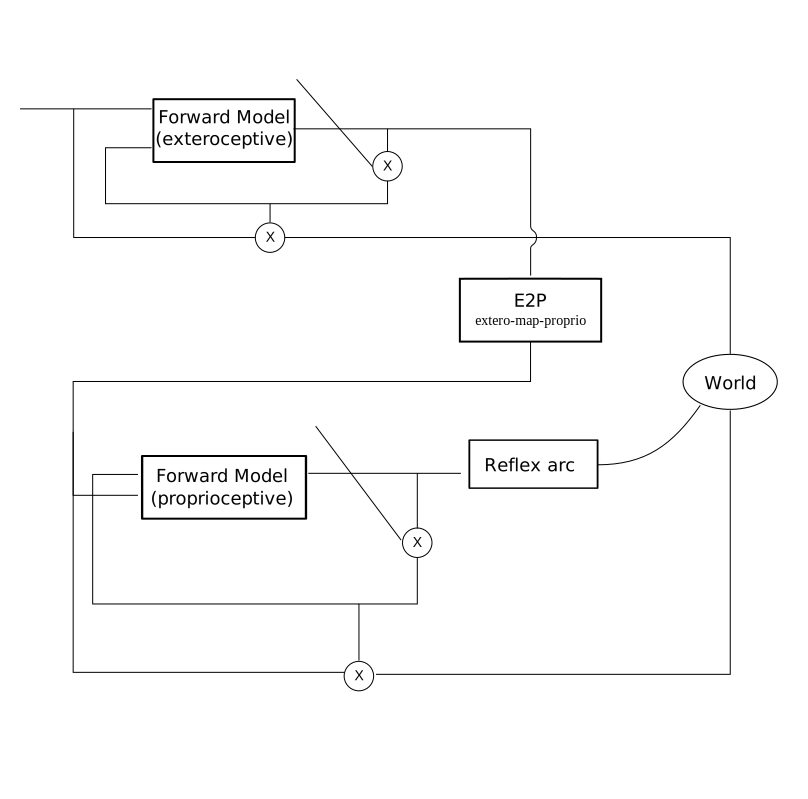
\includegraphics[width=0.99\textwidth]{img/actinf_large_diagram_p_e2p_e.pdf}
  \caption{Hello grpahicxs}
\end{figure}

\subsection{Propio-Extero Mapping Model}
\label{subsec:exteropropio}


There would be here, the part that Guido was implementing on the forming of trajectories.




%%%%%%%%%%%%%%%%%%%%%%%%%%%%%%%%%%%%%%%%%%%%%%%%%%%%%%%%%%%%%%%%%%%%%%%%%%%%%%%%
\section{Notes}
\label{sec:org863d8de}

\subsection{control theory parallels}
\label{sec:org316353f}

i don't see this as a problem at all, to the contrary, it means if you
arrive at a model setup you can actually look to adaptive control and
translate the solution to your formulation.

in terms of the philosophy see email from \textit{<2016-10-11 Di> } so it's
clearly about a different issue.

\subsection{merge bruno's initial draft}
\label{sec:org6e00d89}


\subsection{opt's notes}
\label{sec:org35938d1}
\begin{itemize}
\item for proprio-only show 3 figures: 1) behaviour without any learning,
which fails to precisely reach the goals because proprio
predictions don't "match" proprio states (nonlinear
deformations), 2) behaviour during learning, see how we actually
move closer to the goal over a few timesteps, 3) behaviour while
still learning but going to places we have already been: no error,
no learning / weight changes
\item additional plots: original timeseries, model sweep response plot
\end{itemize}

%% %%%%%%%%%%%%%%%%%%%%%%%%%%%%%%%%%%%%%%%%%%%%%%%%%%%%%%%%%%%%%%%%%%%%%%%%%%%%%%%%
%% \section{Introduction}
%% \label{sec:orga5a5ee2}


%%%%%%%%%%%%%%%%%%%%%%%%%%%%%%%%%%%%%%%%%%%%%%%%%%%%%%%%%%%%%%%%%%%%%%%%%%%%%%%%
\section{Experiments}
\label{sec:org347db7c}

  \begin{itemize}
  \item deploy models to different robotic systems: Nao, SimpleArm,
    Pointmass, two-wheeled
  \item timeseries analysis
  \item learning transient (arbitrarily fast, see Tin + Poon)
  \item explicitly map out the acquired models by sweeping the inputs and
    record their outputs
  \item what happens under perturbation?
  \item long-term adaptation effects: are we only plastic or are we also
    stable? do new adaptations overwrite previous ones? does a given
    approximator become saturated (just think how critical weight
    initialization in neural networks can be) in terms of its adaption
    capacity?, can be enforced via decay schedules of learning rate
    etc
  \end{itemize}


%%%%%%%%%%%%%%%%%%%%%%%%%%%%%%%%%%%%%%%%%%%%%%%%%%%%%%%%%%%%%%%%%%%%%%%%%%%%%%%%
\section{Discussion}
\label{sec:orga3d6260}

Discuss, compare with existing approaches like std fwd/inv model
  pairs or reinforcement learning

%%%%%%%%%%%%%%%%%%%%%%%%%%%%%%%%%%%%%%%%%%%%%%%%%%%%%%%%%%%%%%%%%%%%%%%%%%%%%%%%
\section{Summary}
\label{sec:orgc71dbe7}



\printbibliography
\end{document}


